
\chapter{What is the story of Green Buddhism?}
\epigraph{If scientific analysis were conclusively to demonstrate certain claims
in Buddhism to be false, then we must accept the findings of science and abandon
those claims.}
{Dalai Lama XIV\cite{singleAtom}}
\label{whatstory}
In 2009 I went to Thailand to be a monk for a month. I liked the robes but they
said I couldn't wear them when I got back to Canada, unless I was a monk at one
of their temples. However when I asked if I could remake them into a different 
colour, like green or purple and then wear them, they said sure. 

\begin{figure}
  \centering
  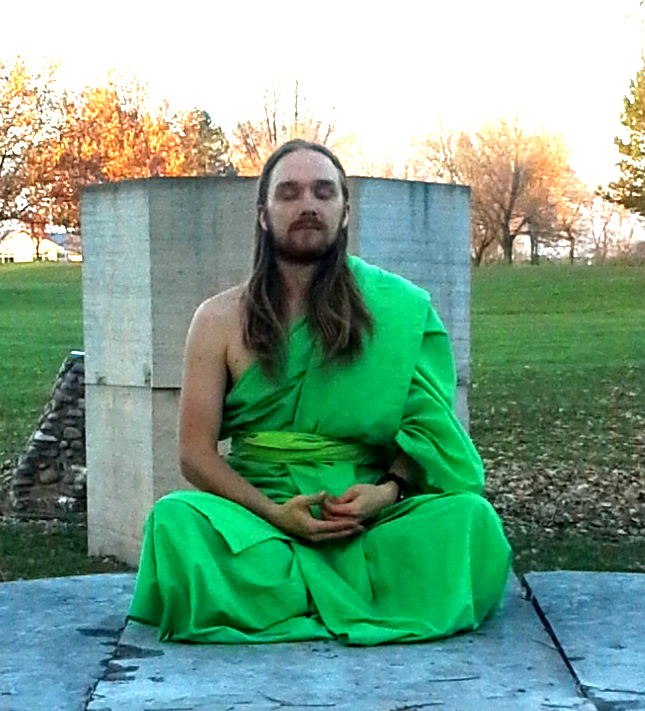
\includegraphics[width=0.61\textwidth]{photograph/logan_streondj_meditating_20151109.png}
  \caption{Logan Streondj meditating in a henge, Kelso Beach, 
          Owen Sound, Ontario, Canada}
\label{fig:meditating}
\end{figure}

The robe style has been around for thousands of years, and is used by a variety
of different faiths in Asia. 

Also while I was in Thailand, I was somewhat disenchanted, or even frightened by
the blatant disregard for nature. When I asked to go to a park, the only
greenspace in the town of Fang, was the cemetery. 

I returned to Canada and turned to gardening, and earth-based religion for a
while. I ride a bike, am vegan, eat organic, and various other ``green''
practices.

Buddhism as the opening quote shows, is the most science like of all religions,
so I keep coming back to it. 

In 2015 I moved to Owen Sound, and tailored myself a green Buddhist
robe (\ref{fig:meditating}). So
other than my inclinations for environmentalism, I also attend regular Buddhist
meditation gatherings in my robes.

Earlier, in 2006, I was doing a hermitage in my parents basement. Only writing
my thoughts and meditating for a year, with minimal contact with the outside
world. I achieved many deep states of meditation.  

One of which was that of emptiness, a delta brainwave meditation. 
I came to a certain understanding of nothingness, and the origin of the
cosmos (\ref{origination}).

The profound realization of my awakening, is that truth is personal, and that
reality is mutual. When attempting to explain it to someone, they said it was
the basis for a religion. 

Indeed it has been. To define a word, one could make a dictionary entry. Though
I decided to go the path of creating a human speakable programming language.
Humans having liquid minds, which  may flow into other definitions. Once a word
is defined in computer programming, it can be a foundation of a whole genus of
minds, solid as can be.  

In addition to my vision of the origins of the cosmos, and profound
realizations, I also had many visions of my past lives. Of course they are only
my truth, so you don't have to believe them, to you they are only imaginary
stories. 


\blockquote[Kalamas Sutta\cite{kalamas}]{Now, Kalamas, don't go by reports, by legends, by traditions, 
by scripture, by logical conjecture, by inference, by analogies, by agreement 
through pondering views, by probability, or by the thought, ``This contemplative
 is our teacher.'' When you know for yourselves that, ``These qualities are 
skillful; these qualities are blameless; these qualities are praised by the 
wise; these qualities, when adopted and carried out, lead to welfare and 
to happiness'' — then you should enter and remain in them.
}

In my alleged past lives, I've traveled between galaxies, and reincarnated in a
great variety of solid, liquid and even gaseus bodies. My vision, is to see the
co-operation of all. So we may all live with safety, health, socializing, and
liberty. 

Summarizing What is Green Buddhism?
\begin{itemize}
  \item Green as in ecological friendliness.
  \item Green as in the colour of this Buddhist school's robes. 
  \item Buddhism as in meditation gatherings. 
  \item Buddhism as in the most science friendly
religion\cite{kalamas}\cite{singleAtom}. 
  \item Religion as in an operating-system.
\end{itemize}
